\documentclass{article}

\usepackage{nips_2018_author_response}

\newcommand*{\firstdraft}{4 November 2015}
\newcommand*{\published}{22 May 2018}

\newcommand*{\pdftitle}{Response to reviewers}

\newcommand*{\headtitle}{\pdftitle} %\newcommand*{\pdfauthor}{P.G.L.  Porta Mana, V. Rostami, E. Torre, Y. Roudi}

\usepackage[T1]{fontenc} 
\input{glyphtounicode} \pdfgentounicode=1
\usepackage[utf8]{inputenx}
\newcommand*{\bmmax}{3} % reduce number of bold fonts, before bm
\newcommand*{\hmmax}{0} % reduce number of heavy fonts, before bm
\usepackage{textcomp}
\usepackage{amsmath}
\usepackage{mathtools}
\setlength{\multlinegap}{0pt}

\usepackage{amssymb}
\usepackage{amsxtra}

\usepackage[british]{babel}\selectlanguage{british}
\newcommand*{\langfrench}{\foreignlanguage{french}}
\newcommand*{\langgerman}{\foreignlanguage{german}}
\newcommand*{\langitalian}{\foreignlanguage{italian}}
\newcommand*{\langswedish}{\foreignlanguage{swedish}}
\newcommand*{\langlatin}{\foreignlanguage{latin}}
\newcommand*{\langnohyph}{\foreignlanguage{nohyphenation}}

\usepackage[autostyle=false,autopunct=false,english=british]{csquotes}
\setquotestyle{british}
\usepackage{bm}



\usepackage[shortlabels,inline]{enumitem}
\SetEnumitemKey{para}{itemindent=\parindent,leftmargin=0pt,listparindent=\parindent,parsep=0pt,itemsep=\topsep,topsep=0pt}
% \begin{asparaenum} = \begin{enumerate}[para]
% \begin{inparaenum} = \begin{enumerate*}
\setlist[enumerate,2]{label=\alph*.}
\setlist[enumerate]{leftmargin=1.5em,topsep=-1ex}
\setlist[itemize]{leftmargin=1.5em}
\setlist[description]{leftmargin=\parindent}

%% With euler font cursive for Greek letters - the [1] means 100% scaling
\DeclareFontFamily{U}{egreek}{\skewchar\font'177}%
\DeclareFontShape{U}{egreek}{m}{n}{<-6>s*[0.95]eurm5 <6-8>s*[0.95]eurm7 <8->s*[0.95]eurm10}{}%
\DeclareFontShape{U}{egreek}{m}{it}{<->s*[0.95]eurmo10}{}%
\DeclareFontShape{U}{egreek}{b}{n}{<-6>s*[0.95]eurb5 <6-8>s*[0.95]eurb7 <8->s*[0.95]eurb10}{}%
\DeclareFontShape{U}{egreek}{b}{it}{<->s*[0.95]eurbo10}{}%
\DeclareSymbolFont{egreeki}{U}{egreek}{m}{it}%
\SetSymbolFont{egreeki}{bold}{U}{egreek}{b}{it}% from the amsfonts package
\DeclareSymbolFont{egreekr}{U}{egreek}{m}{n}%
\SetSymbolFont{egreekr}{bold}{U}{egreek}{b}{n}% from the amsfonts package
% Take also \sum, \prod, \coprod symbols from Euler fonts
\DeclareFontFamily{U}{egreekx}{\skewchar\font'177}
\DeclareFontShape{U}{egreekx}{m}{n}{%
       <-7.5>s*[0.9]euex7%
    <7.5-8.5>s*[0.9]euex8%
    <8.5-9.5>s*[0.9]euex9%
    <9.5->s*[0.9]euex10%
}{}
\DeclareSymbolFont{egreekx}{U}{egreekx}{m}{n}
\DeclareMathSymbol{\sumop}{\mathop}{egreekx}{"50}
\DeclareMathSymbol{\prodop}{\mathop}{egreekx}{"51}
\DeclareMathSymbol{\coprodop}{\mathop}{egreekx}{"60}
\makeatletter
\def\sum{\DOTSI\sumop\slimits@}
\def\prod{\DOTSI\prodop\slimits@}
\def\coprod{\DOTSI\coprodop\slimits@}
\makeatother

\usepackage{mathdots}
\usepackage{microtype}

\iffalse
\usepackage[backend=biber,mcite,subentry,citestyle=numeric-comp,bibstyle=numericbringhurst,autopunct=false,sorting=none,sortcites=false,natbib=false,maxnames=8,minnames=8,giveninits=true,block=space,hyperref=true,defernumbers=false,useprefix=true,language=british]{biblatex}
\renewcommand*{\finalnamedelim}{, }
\setcounter{biburlnumpenalty}{1}
\setcounter{biburlucpenalty}{0}
\setcounter{biburllcpenalty}{1}
\DeclareDelimFormat{multicitedelim}{\addsemicolon\space}
\DeclareDelimFormat{postnotedelim}{\space}
\addbibresource{portamanabib.bib}%comment for arxiv
\renewcommand{\bibfont}{\footnotesize}
%\defbibheading{bibliography}[\bibname]{\section*{#1}\addcontentsline{toc}{section}{#1}%\markboth{#1}{#1}
%}
\newcommand*{\citep}{\parencites}
\newcommand*{\citey}{\parencites*}
\renewcommand*{\cite}{\citep}
\providecommand{\href}[2]{#2}
\providecommand{\eprint}[2]{\texttt{\href{#1}{#2}}}
\newcommand*{\amp}{\&}

\newcommand*{\arxiveprint}[1]{%\global\def\arxivp{\arxivsi}%\citeauthor{0arxivcite}\addtocategory{ifarchcit}{0arxivcite}%eprint
\texttt{\urlalt{https://arxiv.org/abs/#1}{arXiv:\hspace{0pt}#1}}%
%\texttt{\href{http://arxiv.org/abs/#1}{\protect\url{arXiv:#1}}}%
%\renewcommand{\arxivnote}{\texttt{arXiv} eprints available at \url{http://arxiv.org/}.}
}
\newcommand*{\mparceprint}[1]{%\global\def\mparcp{\mparcsi}%\citeauthor{0mparccite}\addtocategory{ifarchcit}{0mparccite}%eprint
\texttt{\urlalt{http://www.ma.utexas.edu/mp_arc-bin/mpa?yn=#1}{mp\_arc:\hspace{0pt}#1}}%
%\texttt{\href{http://www.ma.utexas.edu/mp_arc-bin/mpa?yn=#1}{\protect\url{mp_arc:#1}}}%
%\providecommand{\mparcnote}{\texttt{mp_arc} eprints available at \url{http://www.ma.utexas.edu/mp_arc/}.}
}
\newcommand*{\philscieprint}[1]{%\global\def\philscip{\philscisi}%\citeauthor{0philscicite}\addtocategory{ifarchcit}{0philscicite}%eprint
\texttt{\urlalt{http://philsci-archive.pitt.edu/archive/#1}{PhilSci:\hspace{0pt}#1}}%
%\texttt{\href{http://philsci-archive.pitt.edu/archive/#1}{\protect\url{PhilSci:#1}}}%
%\providecommand{\mparcnote}{\texttt{philsci} eprints available at \url{http://philsci-archive.pitt.edu/}.}
}
\newcommand*{\biorxiveprint}[1]{%\global\def\biorxivp{\biorxivsi}%\citeauthor{0arxivcite}\addtocategory{ifarchcit}{0arxivcite}%eprint
\texttt{\urlalt{http://biorxiv.org/content/early/#1}{bioRxiv:\hspace{0pt}#1}}%
%\texttt{\href{http://arxiv.org/abs/#1}{\protect\url{arXiv:#1}}}%
%\renewcommand{\arxivnote}{\texttt{arXiv} eprints available at \url{http://arxiv.org/}.}
}
\newcommand*{\osfeprint}[1]{%
\texttt{\urlalt{https://doi.org/10.17605/osf.io/#1}{doi:10.17605/osf.io/#1}}%
}
\fi

\usepackage{graphicx}

\PassOptionsToPackage{hyphens}{url}\usepackage[hypertexnames=false]{hyperref}
%\usepackage[depth=4]{bookmark}
\hypersetup{colorlinks=true,bookmarksnumbered,pdfborder={0 0 0.25},citebordercolor={0.2 0.1333 0.5333},%bluish
citecolor=mybluishpurple,linkbordercolor={0.0667 0.4667 0.2},%greenish
linkcolor=mypurplishred,urlbordercolor={0.5333 0.1333 0.3333},%reddish
urlcolor=mygreen,breaklinks=true,pdftitle={\pdftitle}}
% \usepackage[vertfit=local]{breakurl}% only for arXiv
\providecommand*{\urlalt}{\href}

\selectlanguage{british}\frenchspacing
% \usepackage{booktabs}       % professional-quality tables
% \usepackage{amsfonts}       % blackboard math symbols
% \usepackage{nicefrac}       % compact symbols for 1/2, etc.
%\usepackage{lipsum}

\begin{document}
We thank the reviewers for their analysis, appreciative words, and
suggestions. We reply to major points only. The manuscript can be easily
amended to address the points we don't discuss here.

\textbf{Reviewer 1}
\begin{enumerate}
\item It would be interesting to use the frequency distribution of the
  sample activity, measured in the recording, as a constraint, equivalent
  to $n$ moment constraints. In fact, using it at the population level is
  less questionable than using at the sample level (activities with zero
  frequencies lead to zeroes in the maximum-entropy distribution, and these
  are unreasonable because the sample size is much smaller than the
  state-space size. This indicates that maximum-entropy is used beyond its
  range of validity). Its use, however, addresses a different question than
  the one discussed in our introduction, namely to define and measure
  \enquote{cooperativity} by comparing maximum-entropy distributions
  constructed from different numbers of moments.
\item It's true, we forgot to discuss how the population-level application
  solves the sample-size-dependence of maximum-entropy results pointed out in
  previous literature. This should be addressed in an amended version of
  the paper.
\end{enumerate}

\bigskip

\textbf{Reviewer 2}
\begin{enumerate}
\item We agree that the comparison with other approaches is important. But
  we believe that it's also important to carefully examine (1) the question
  we're asking, and (2) which first principles can be used to translate it
  into a mathematical problem. Some literature develops very refined --
  though often ad hoc -- mathematical techniques, but then leaves us
  unsatisfied, with the lingering question \enquote{why were we doing
    this?}. This is the reason for our long introductory discussion about
  the problem and the first principles that can be used to address it.
\item The firing rate likely affects the results and the quantification of
  \enquote{cooperativity}. Is this an issue? is our idea of
  \enquote{cooperativity} invariant with respect to the firing rate, or
  not? Requirements of this kind constrain the translation of cooperativity
  into a mathematical quantity. This again shows the importance of defining
  the question we're asking first.
\item Regarding correlations: the method quantifies cooperativity using the
  measured correlations; see the \enquote{protocol} 1--3 in the
  Introduction. Thus, correlations determine the result.
\item We agree that there are many approaches in the literature. In the
  literature we have explored we've seen very little use of the basic
  sampling formulae presented in our paper. Honestly this surprised us,
  because they're surely essential even in a very basic analysis of the data.
\end{enumerate}

\bigskip

\textbf{Reviewer 3}
\begin{enumerate}
\item We agree with the Reviewer that the main formulae of the paper, (17)
  and (19), probably have little \emph{experimental} use today. But the
  formulae and the analysis behind them are important exactly for the
  points raised by the Reviewer:
  \begin{itemize}
  \item \begin{minipage}[t]{0.74\linewidth}The Reviewer says \enquote{the
        differences between the sample level and population level
        distribution seem minor}: this could be true, but we could not have
      known this, if we hadn't faced the whole problem and derived a
      formula showing that the difference is minor.
    \end{minipage}\hspace{\fill}
    \smash{\begin{minipage}[t]{0.24\linewidth}\vspace{0pt}
      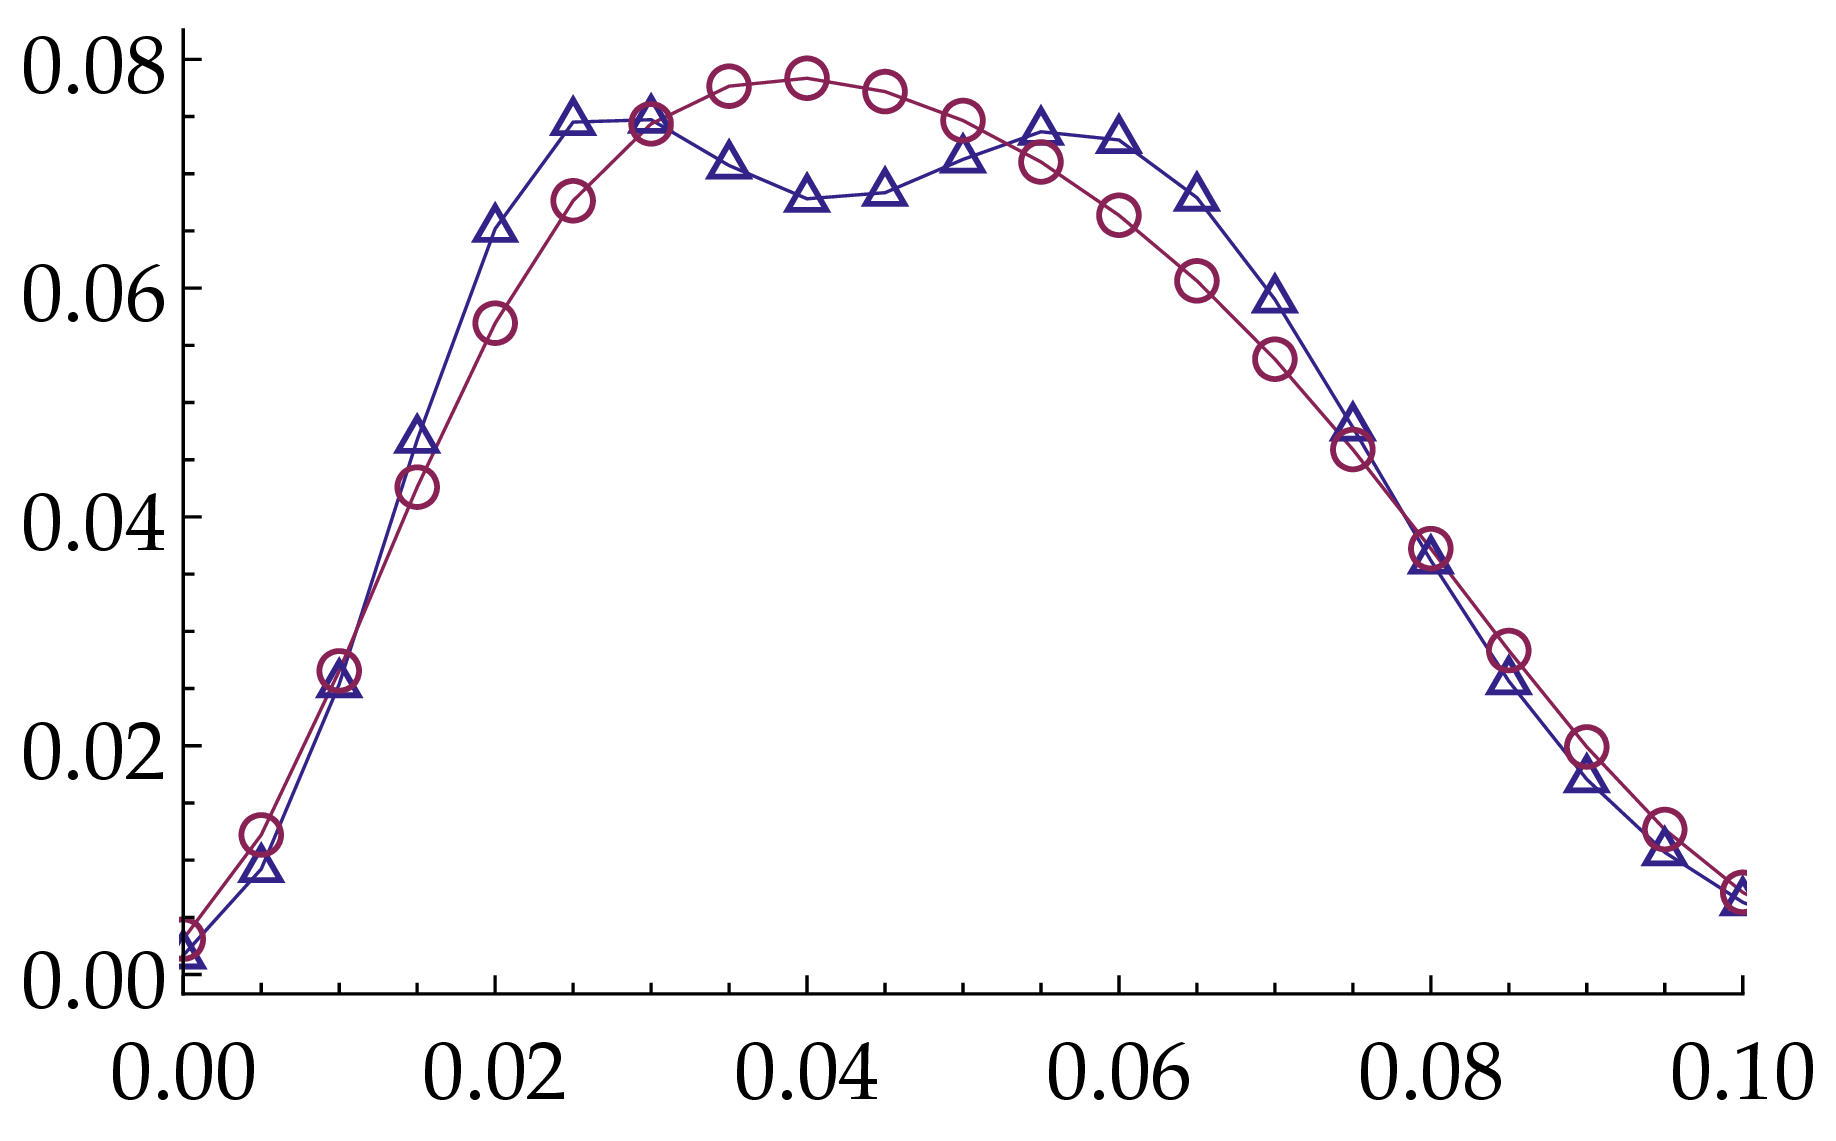
\includegraphics[width=\linewidth]{zoom_4mom.png}
    \end{minipage}}
  \item
    \begin{minipage}[t]{0.74\linewidth}
      Application of the method with higher-order constrains can show more
      interesting differences between sample- and population-level
      distributions. See e.g. the plot on the right: the bimodal
      distribution is the marginalized, population-level one.
    \end{minipage}
%     % \setlength{\intextsep}{0.5ex}% with wrapfigure
%     \begin{figure}[h!]%{r}{0.4\linewidth} % with wrapfigure
%   \centering
% %\caption{***}\label{fig:comparison_a5}
% \end{figure}
\item Calculations show that the population-level distribution can be less
  or more entropic than the sample-level one. But a more entropic
  distribution is not necessarily more correct (we could just use a uniform
  distribution then). The question is how the constraints are appropriately
  applied in the method. 
\end{itemize}
As this Reviewer and Reviewer 2 remark, the points and findings above
deserve more discussion. Unfortunately there are space constraints, and we
preferred to give more room to a careful analysis of the principles behind
the method, to see whether the method is correctly applied. Our main wish
is that our readers will give more thoughts to these matters. We could
hurry up and produce a lot of mathematical results; but, whether positive or
negative, such would be meaningless if the method isn't meaningfully
applied. And it isn't always the case that a meaningful application of a
method can be judged by its results alone.
% \item We agree with Reviewer 3 that the paper emphasizes some philosophical
%   aspects; intentionally so. Sadly we can't make all kinds of readers
%   happy; a choice of audience is necessary. As readers ourselves we
%   appreciate when a paper begins by asking: \enquote{What is the question?
%     is it possible to translate it into a mathematical problem? which
%     principles can we use to make such translation?}. There are papers that
%   develop very refined mathematical techniques but leave us unsatisfied,
%   with the lingering question \enquote{why are we doing this?}. This is the
%   reason why we try to emphasize these kinds of questions. But we are sure
%   that part of the NIPS audience will appreciate this emphasis.
\end{enumerate}
\end{document}
